% book example for classicthesis.sty
\documentclass[10pt,a6paper,footinclude=false,firstfoot=false,headinclude=true,open=any,DIV=6]{scrbook} % KOMA-Script book
\usepackage[paperheight=5.5in, paperwidth=4.25in]{geometry}
\usepackage[T1]{fontenc}                
\usepackage{lipsum}
\usepackage[pdfspacing,manychapters]{zine}
\usepackage{cmzine}
\usepackage{amsthm}
\usepackage{ellipsis}
\usepackage{xcolor}
\usepackage{graphicx}
\usepackage{changepage}
\usepackage{wrapfig}
\usepackage{xfrac}
% \usepackage{poemscol}
\usepackage{verse}
\usepackage{enumitem}
% \usepackage{showframe}
% \usepackage{layouts}

%set font to anttor
    \usepackage[light,math]{anttor}

% set font to Calligra
    \usepackage{calligra}
    
    
    % \usepackage{tgpagella}

%sets font to Gentium
    \usepackage[T1]{fontenc}
    \usepackage{bookman}



\begin{document}

\thispagestyle{empty}
\hbox{}
\newpage
\pagenumbering{gobble}
    
%begin title page
    \setcounter{page}{1}
    % \newgeometry{left=.7cm, right=0cm, top=5cm}
    \newgeometry{left=1cm, right=1cm, top=5cm}
    \thispagestyle{empty}
    \pagecolor{geraniumTitleColor}
   
    
    % \hspace{-.3em}\inTitleCalligra{Fern}\hspace{-1.1em}\inTitleCaps{fern}
    
    % \hspace{1.6em}\inTitleDate{July \texttt{\^} August}
    
    % \hspace{-2em}\inTitleCalligra{Days}\hspace{-1.78em}\inTitleCaps{geranium}
    
    \begin{center}
    \inTitleCaps{balsam root}
    
    \noindent\inTitleDate{July \texttt{\^} August}
    \end{center}
   
%end title pages    
    \newpage
    \pagecolor{white}
    % \cleardoublepage
    \restoregeometry
    \normalfont
    \normalsize
    \color{black}
    
    \pagenumbering{gobble}
    \setcounter{page}{2}
    
\chapter{welcome to balsamroot}

% \pagevalues

		
So what is this? It's a zine. Which is to say it is a small magazine. This zine in particular is filled with the life of Michelle and Chris and hopefully the rest of the people those two love. To quote Brett and Lindie, ``this is for us.''

We hope that this can be a way for us all to share with each other some things about our lives. In this issue, for example, Michelle and I share some things we're reading and listening to, a poem, and a nice recipe for making yogurt in the fashion of DIY.

While this issue of \spacedlowsmallcaps{balsamroot} is heavy on the M \& C lifestyle that's only because you guys didn't know that you were supposed to submit things for it. In the future that can be different. So here we call to y'all to send us thoughts, recipes, songs, diagrams of wood working projects, drawings of small creatures, descriptions of beautiful scenery, calls to action, elegies, and anything else about your life.

It's a social media. But the media is paper. \initials{L}{Y}
\vspace{1ex}

\noindent{\color{halfgray} \spacedlowsmallcaps{PS} \footnotesize Oops, we got a little delayed putting this all together. Anyway, here is what we were doing this summer.}

\tableofcontents 

\newpage
% \thispagestyle{empty}
% \hbox{}
% \cleardoublepage
\pagenumbering{arabic}
\setcounter{page}{2}

\raggedbottom
    

\chapter{do you like hobbies?}

\spacedlowsmallcaps{What we're listening to}:

\par\noindent\ignorespaces\album{Crack_Up}{Crack-Up}{Fleet Foxes}{You know how Fleet Foxes is about having a beard and being in the forest and falsettos and harmonizing? This album is about how sometimes in life that doesn't work out. The namesake of a series of essays from F. Scott Fitzgerald, this album is complex, shifting, and ultimately uplifting. \initials{C}{G}}

\album{PaulSimon}{paul simon}{Paul Simon}{Listening to Paul Simon's self titled album produces the same homey, Saturday Morning Breakfast feelings as Crosby, Stills \& Nash but adds to the folksy, bluesy soft rock with international influences from Jamaica and South America. \initials{M}{Y}}

\album{Meeting_of_the_Waters_cover}{Meeting of the Waters}{Animal Collective}{Recorded in the Amazon jungle with some new Viceland show, this EP is filled mostly with the sounds of the jungle and slow, quiet singing---and maybe a washing machine. Listen to the second track, \textit{Man of Oil}, for the pop hit. \initials{C}{G}}

\vspace{2ex}
\titlerule

\vspace{2ex}
\noindent\spacedlowsmallcaps{What we're reading}:
\vspace{1ex}

\book{life is elsewhere}{Milan Kundera}
Milan Kundera is always a good read for when you want to read a novel that is heavy on reflection and philosophy and you want to know that it's heavy on reflection and philosophy. Here we get a look at the life of the ``poet'' in that tumultuous, glorious time of communist revolution in Czechoslovakia. Basically it's a commentary on how empty and vapid and self-involved young revolutionary poets are. Lots of lofty ideals and youthful naivete (poets being necessarily naive, as only by inexperience can they truly grasp the emotion of life) which create a great framework for looking at revolution and art and the limits of ourselves. It's like Rilke's \textit{Letters to a Young Poet} through the eyes of the poet and without the sagacious mentor. \initials{C}{G}

\chapter{Making yogurt in paraguay}

When I moved to Coronel Martinez, about four months ago now, the first person I met was Christina, a 35 year old woman of great vitality who sold milk and cheese from her four cows. Christina and I  would chat for hours while she worked, washing clothes and preparing lunch for her husband and two sons. We would think up new project ideas for our gardens or she would explain to me the processes of pasteurizing milk or culturing cheese. We quickly became close friends as I was eager to learn more about her small dairy and we were stimulated by scheming up and carrying out new ideas for her homestead.
 
One of our first ideas was to learn how to make yogurt together; she already had a source of milk and her family loved to drink yogurt in the hot summer evenings. Having homemade yogurt would be beneficial for them because it contains less sugar than the yogurt from the store and it has more probiotics. Our plan was to first make yogurt for her family and myself and then develop a way to produce it in large quantities to be sold  to the 20 families who were already buying her milk and cheese.
 
One sweltering afternoon while Christina and I were chatting and drinking \textit{terere} in her cozy, brick kitchen we realized that we had gathered enough information from friends and YouTube videos to start our first yogurt trial. With care, we boiled the milk, mixed it with the yogurt starter, and waited anxiously. Unfortunately, that night I left her house disappointed because after waiting for six hours our ``yogurt'' still resembled milk.
 
The next morning I got a call from Chris\-tina. \textit{``Mich\-elle, sa\-bes que?''} she said to me. \textit{``Estoy com\-iendo yo\-gur.''} Our yogurt had taken over fourteen hours to thicken but overnight it had turned into a creamy treat, ready to be served with fruit or granola. We were overjoyed and inspired to perfect our recipe.
 
We entered late summer with a routine of preparing a liter of yogurt about once a week, each time making small changes to the recipe so that the yogurt culture would reproduce more rapidly. Once we had a better practical grasp of the recipe, we started to flavor the yogurt with bananas from her trees and canned peaches. We decided to buy strawberry plants with hopes of flavoring the yogurt with homegrown strawberries in the spring.
 
Now that autumn is upon us, I've found that the mornings almost require hot oats or toast rather than fruity yogurt smoothies. The strawberry plants have been waiting anxiously to be transplanted out of their tiny \textit{macetas}. Christina's cows are starting to produce less milk every day and will soon enter into a non-lactating period. For the coming spring, my hopes are that we will recall our cravings for yogurt and be blessed with handfuls of tiny red fruits every \mbox{day.\initials{M}{Y}}

\section*{Christina \& Michelle's Yogurt Recipe}

\hspace{1em}\spacedlowsmallcaps{What you'll need}:
\vspace{2ex}

\noindent\hspace{1em}
\mbox{
    \hspace{-1em}
    \begin{minipage}[t]{0.225\textwidth}
        \centering
        
\includegraphics[width=0.5\textwidth]{Ing1}
        
        \sfrac{1}{2} cup plain yogurt (starter)
    \end{minipage}
    \begin{minipage}[t]{0.225\textwidth}
        \centering
        
\includegraphics[width=0.5\textwidth]{Ing2}
        
        1 liter whole milk
    \end{minipage}
    \begin{minipage}[t]{0.225\textwidth}
        \centering
        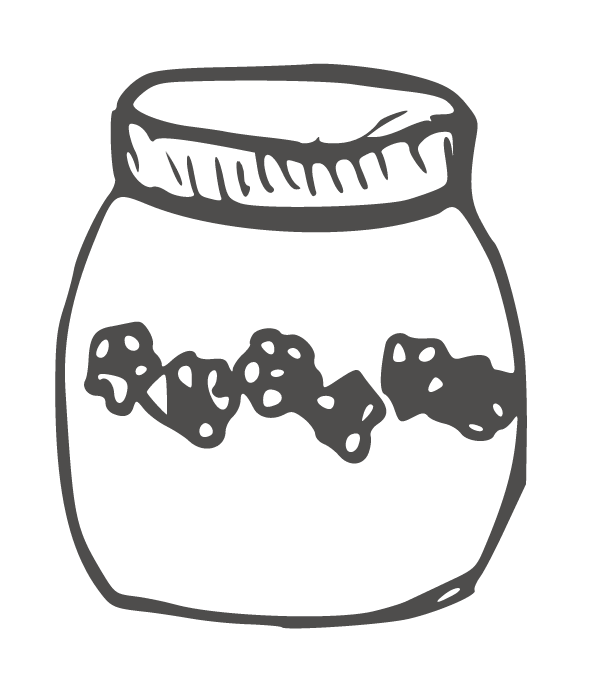
\includegraphics[width=0.5\textwidth]{Ing3}
        
        1 \sfrac{1}{2} liter container with lid
    \end{minipage}
    \begin{minipage}[t]{0.225\textwidth}
        \centering
        
\includegraphics[width=0.5\textwidth]{Ing4}
        
        Sunny/warm spot and blanket
    \end{minipage}
}

\vspace{4ex}


\recipeStep{Step1}{Heat milk to 42$^{\circ}$ C or a little warmer than skin temperature. This is the ideal temperature for yogurt bacteria reproduction.}

\recipeStep{Step2}{Splash a little milk into the container and mix well with the yogurt.}

\vspace{1em}

\recipeStep{Step3}{Add the remaining warm milk.}\vspace{1em}

\recipeStep{Step4}{Screw on the lid and wrap the container in a blanket. Place in a warm or sunny spot to keep the mixture as close to 42$^{\circ}$ C as possible.}

\vspace{3ex}

\begin{minipage}{\linewidth}\noindent\hspace{1em} Four to five hours later... yogurt!
\begin{center} 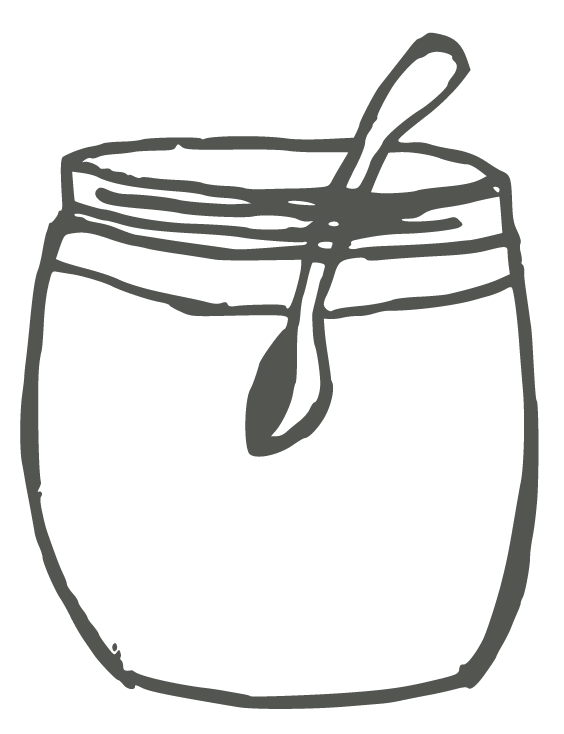
\includegraphics[width=0.15\textwidth]{Final} 
\end{center}
\end{minipage}

\chapter{the wind is enough to compete with}

\begin{verse}
I am a pigeon's flutter captured at 1/50 \\
enough to grab a feather and lose it again in the fury 

Wind is falling from beneath my fingernails \\
and I find it hard to keep these papers flat \\
They flutter and fall \\
The worst are those which slip \\
into the crack at the back of my desk \\
That crack goes way down \\
I've tried to squeeze back there myself \\
for, I believe, a letter that I couldn't bear to part with \\
From my grandmother or a lover \\
I'm lost, I told you \\
it's a slit to forever \\
and my body can't go or my memories \\
only my damned words 

The wind's in my eyes now \\
so the rain's there too getting blown sideways \\
the kind of storm you hold your head down against \\
and your coat close to your chest \\
both arms crossed against one another \\
and your papers pushed down into the safe warm spot above your lungs \\
and the rain drives against your back \\
and over there towards that crack. \initials{C}{G}
\end{verse}

\vspace{1em}
\begin{center}
\noindent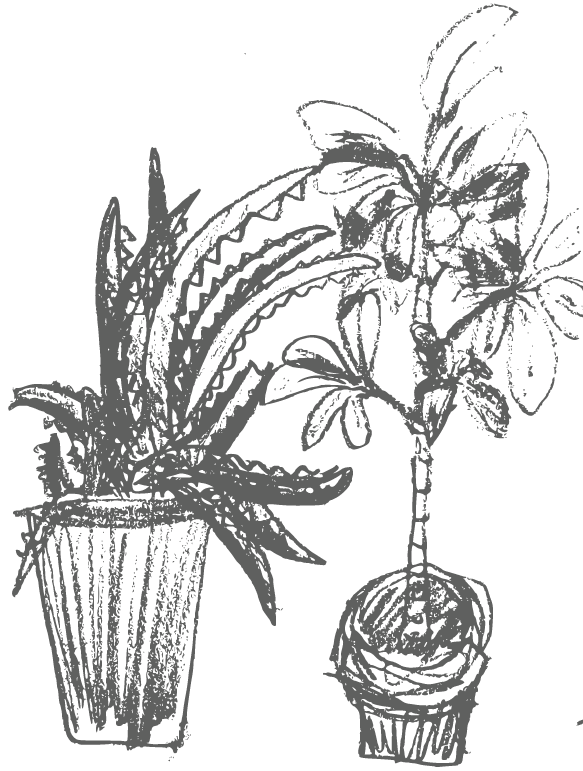
\includegraphics[width=0.5\textwidth]{FernsVec.png}
\end{center}


\chapter{Recipe: Spiced Pear Bread}

I love this spiced up banana bread recipe on a cold autumn morning with a cup of coffee. The pure flavor of pears provide the perfect medium for all the spices you would find in a cup of chai. Try replacing pears in the recipe with other fruits you may have on hand, but be careful, extract the milk from the recipe when using more liquid fruits like pureed banana.

\vspace{2ex}
\spacedlowsmallcaps{What you'll need}:

\setlist[description]{labelindent=2em}
\begin{description}
\item [\sfrac{1}{2} cup] granulated sugar
\item [\sfrac{1}{4} cup] molasses or honey
\item [1 stick] softened butter
\item [2] eggs
\item [1 teaspoon] vanilla extract
\item [2 teaspoons] baking powder
\item [2 teaspoons] cinnamon
\item [\sfrac{1}{2} teaspoon] finely chopped ginger
\item [\sfrac{1}{4} teaspoon] ground nutmeg
\item [1 dash] of  ground cardamom
\item [1 dash] of ground cloves
\item [1 dash] of black pepper
\item [\sfrac{1}{2} teaspoon] salt
\item [\sfrac{1}{2} cup] milk
\item [2] diced pears
\item [1 cup] all-purpose flour
\item [1 cup] whole-wheat flour
\item Cinnamon \& sugar for sprinkling on top
\end{description}

Preheat oven to 400$^{\circ}$ F. Cream sugar, honey, and butter. Add eggs and vanilla. Stir in baking powder, spices, and salt. Then mix in the milk and diced pears. Finally add the flours a little at a time while stirring. Pour mixture into a greased pan and sprinkle with cinnamon and sugar. Place in the oven for about half an hour or until a knife leaves clean. Enjoy! \initials{M}{Y}

\chapter{How's your garden growing?}

Living in a swamp has cool benefits like snails and butterflies that come in through the windows at night. However, gardening in such humidity would be quite problematic so instead, I decided to create green spaces on top of the cement that surrounds my house. I had a carpenter make a 1x2 meter bed where I've used square foot gardening to optimize the number of plants without inhibiting plant growth. I recommend this system for anyone working with limited space. I obtained three old wash bins where carrots, beets, yarrow and chamomile are flourishing. I've found that soil depths aren't critical when the plants are sown in healthy soil.

I was able to fit two climbing spinach, one eggplant, one bell pepper, eight swiss chard, five kale, one cauliflower, and one zucchini.
I planted my herbs in a pallet because their roots are more shallow.
To create the soil, I mixed old cow poop with sand and dirt with a ratio of 2:1:1 respectively. \initials{M}{Y}

\begin{center}
\noindent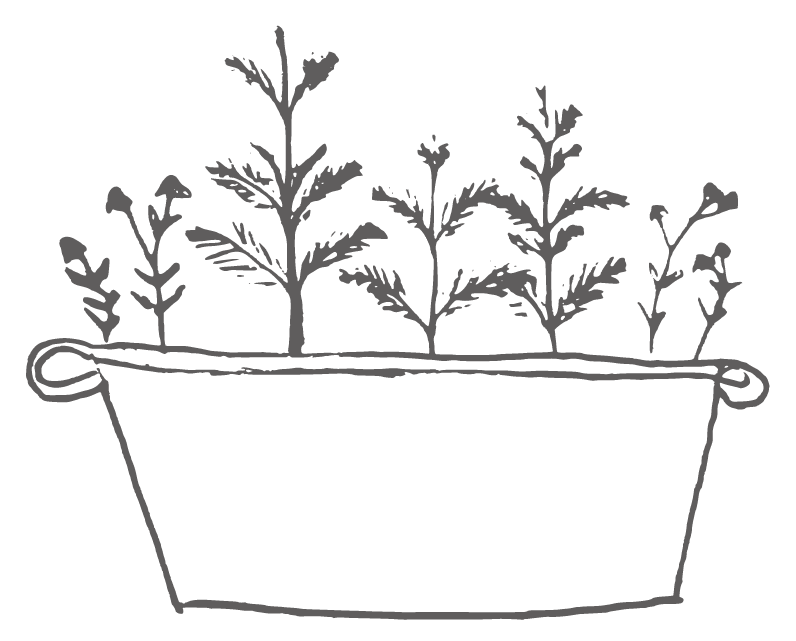
\includegraphics[width=0.6\textwidth]{MichGardenImproved.png}
\end{center}
\vspace{1ex}

I also found myself working my garden into a few small plots this summer. The house I live in has three little raised beds into which I sewed haphazardly. Peas planted at the back edge of the largest bed lent themselves well to a trellis, while climbing cucumbers that I tried to trellis in another bed never took off. Another bed in which I attempted to grow six summer squash and a dozen bush beans wound up growing one and a half squash plants and an assortment of stunted beans. Gold medal goes to the bed of carrots, beans, and radishes which somehow timed out perfectly to never get in each others' way. \initials{c}{g}

\newpage
\thispagestyle{empty}
\newgeometry{left=1cm, right=1cm, top=4cm}

\begin{center}
\begin{minipage}{0.6\textwidth}
\spacedlowsmallcaps{A note on the title:}

\vspace{1em}
\noindent The balsamroot is a genus of flowering plants which grow profusely on the open hillsides of Spokane and the West. Its deep taproot allows it to thrive in arid conditions and the entire plant is edible with many medicinal uses. Its presence is a signifier of the health of the local ecosystem.
\end{minipage}
\end{center}

\end{document}
